\documentclass[12pt,a4paper]{report}
\usepackage[utf8]{inputenc}
\usepackage{amsfonts}
\usepackage{setspace}
\usepackage{graphicx}
\usepackage{array}
\usepackage{fancyhdr}
\linespread{1.5}
\usepackage{geometry}
\geometry{
a4paper,
total={210mm,297mm},
left=1.25in,
right=0.75in,
top=0.75in,
bottom=0.75in,
}

\begin{document}
\pagestyle{empty}
\begin{center}
{\large \textbf{VISVESVARAYA TECHNOLOGICAL UNIVERSITY}}
\par
\vspace{3pt}
{\large \textbf{``JNANA SANGAMA'', BELAGAVI - 590 018}}
\begin{figure}[hbtp]
\centering

\includegraphics[width=0.80in,height=0.75in]{../fig/vtu}
\end{figure}
\\
\textbf{A MINI PROJECT REPORT}
\par
\textbf{on}
\par
\vspace{3pt}
{\Large \textbf{``GRIEVANCE PORTAL MANAGEMENT SYSTEM''}}
\par
\vspace{8pt}
\textit{\textbf{Submitted by}}
\par
\vspace{6pt}
\textbf{\large Srusti Shetty}\hspace{1.65in}\textbf{\large 4SF19IS107}\\
\textbf{\large  Swati}\hspace{2.4in}\textbf{\large 4SF19IS116}\\
\par
\vspace{3pt}
\textit{\textbf{In partial fulfillment of the requirements for the V semester }}
\par
\vspace{0.5pt}
\Large \textbf{DBMS LABORATORY WITH MINI PROJECT}
\par
\vspace{0.5pt}
\normalsize \centering \textbf{of}
\par
\vspace{0.5pt}
\large \textbf{BACHELOR OF ENGINEERING }
\par
\vspace{0.5pt}
\textbf{in}
\par
\vspace{0.5pt}
\large \textbf{INFORMATION SCIENCE \& ENGINEERING}
\par
\vspace{2pt}
\textit{\textbf{Under the Guidance of}}
\par
\vspace{2pt}
\textbf{Ms. Jayapadmini Kanchan}
\par
\vspace{0.5pt}
\textbf{\centering \begin{normalsize}
Assistant Professor, Department of ISE
\end{normalsize} }
\par
\vspace{0.5pt}
\normalsize \centering \textbf{at}\\
\begin{figure}[hbtp]
\centering

\includegraphics[width=1.0in,height=0.85in]{../fig/Sahyadri}
\end{figure}
{\LARGE \textbf{SAHYADRI}}
\par
\vspace{6pt}
{\large \textbf{College of Engineering \& Management}}
\par
\vspace{3pt}
{\large \textbf{Adyar, Mangaluru - 575 007}}
\par
\vspace{3pt}
{\large \textbf{2021 - 22}}

\newpage

{\LARGE \textbf{SAHYADRI}}
\par
\vspace{6pt}
{\Large \textbf{College of Engineering \& Management}}
\par
\vspace{3pt}
{\large \textbf{Adyar, Mangaluru - 575 007}}
\par
\vspace{0.25in}
{\large \textbf{Department of Information Science \& Engineering}}
\par
\begin{figure}[hbtp]
\centering
\includegraphics[width=1.0in,height=0.75in]{../fig/sahyadri}
\end{figure}
{\Large \textbf{CERTIFICATE}}
\end{center}
\par
\vspace{0.10in}
\setstretch{1.5}
\noindent This is to certify that the \textbf{Mini Project} entitled \textbf{``Grievance Potal Management System''}  has been carried out by
\textbf{ Srusti Shetty (4SF19IS107)} and \textbf{Swati  (4SF19IS116)}, the bonafide students of Sahyadri College of Engineering \& Management in partial fulfillment of the requirements for the V semester \textbf{DBMS Laboratory with Mini Project (18CSL58)} of \textbf{Bachelor of Engineering in Information Science \& Engineering} of Visvesvaraya Technological University, Belagavi during the year  2021 - 22. It is certified that all corrections/suggestions indicated for Internal Assessment have been incorporated in the report deposited in the departmental library. The mini project report has been approved as it satisfies the academic requirements in respect of mini project work.

\par
\vspace{0.75in}
\setstretch{1.15}
\begin{tabbing}
\hspace{0.1in}---------------------------------------\hspace{0.3in}\=------------------------------\hspace{0.5in}------------------------------\\
\hspace{0.000025in}\textbf{    Ms. Jayapadmini Kanchan}\hspace{0.30in}\textbf{    Mr. Ganaraj K}\hspace{0.9in}\textbf{Dr. Shamanth Rai}\\
\hspace{0.40in}Assistant Professor\hspace{0.8in}Assistant Professor\hspace{0.6in}HOD \& Associate Professor\\
\hspace{0.31in}Dept. of ISE, SCEM\hspace{0.7in}Dept. of ISE, SCEM\hspace{0.8in}Dept. of ISE, SCEM\\

\end{tabbing}

\par
\vspace{0.25in}
\begin{center}
\large \textbf{External Practical Examination:}
\end{center}
\begin{flushleft}
\begin{normalsize}Examiner's Name \end{normalsize}
\hspace{7.5cm}
\begin{normalsize}Signature with Date\end{normalsize}
\end{flushleft}
\par
\vspace{0.05in}
\begin{flushleft}
1. \ldots\ldots\ldots\ldots\ldots\ldots \ldots \hspace{6.8cm}\ldots\ldots\ldots\ldots \ldots\ldots\ldots 
\par
\vspace{0.25in}	
2. \ldots\ldots\ldots\ldots\ldots\ldots \ldots \hspace{6.8cm}\ldots\ldots\ldots\ldots \ldots\ldots\ldots 
\end{flushleft}


\newpage
\begin{center}
{\LARGE \textbf{SAHYADRI}}
\par
\vspace{6pt}
{\Large \textbf{College of Engineering \& Management}}
\par
\vspace{3pt}
{\large \textbf{Adyar, Mangaluru - 575 007}}
\par
\vspace{0.25in}
{\large \textbf{Department of Information Science \& Engineering}}
\par
\begin{figure}[hbtp]
\centering
\includegraphics[width=1.25in,height=1in]{../fig/sahyadri}
\end{figure}
{\Large \textbf{DECLARATION}} 
\end{center}
\par
\vspace{0.10in}
\setstretch{1.5}
\noindent We hereby declare that the entire work embodied in this Mini Project Report titled
\textbf{''Grievance Portal Management System''} has been carried out by us at Sahyadri College of Engineering and Management, Mangaluru under the supervision of \textbf{Ms. Jayapadmini Kanchan} as the part of the V semester \textbf{DBMS Laboratory with Mini Project (18CSL58)} of \textbf{Bachelor of Engineering} in \textbf{Information Science \& Engineering}. This report has not been submitted to this or any other University.\\
\vspace{0.25in}
\begin{flushright}
\textbf{Srusti Shetty (4SF19IS107)}\\
\textbf{Swati (4SF19IS116)}\\
SCEM, Mangaluru \\
\end{flushright}

% For Individuals
%\begin{flushright}
%Place: Mangaluru \hspace{7.8cm} \textbf{Student Name 1}\\
%Date : \hspace{11.7cm}4SF11IS001\\
%V Semester, B.E., ISE\\
%SCEM, Mangaluru\\
%\end{flushright}

\newpage
\pagestyle{plain}
\pagenumbering{roman}
\chapter*{Abstract}
\addcontentsline{toc}{chapter}{\numberline{}Abstract}
This application is used for submitting their grievances to the portal and the service provider provides the desired solution.This application  consists of a user who can post the issues related to fire, Panchayat, municipal and police. It also consists of an admin who controls the service provider and this helps in solving the particular issues. The database has the issues regarding the above stored in them. In the aspect of software, this project uses PHP as the background database. This portal is available to all users and it is very friendly so that the users can drop their complaints without any issues.

\chapter*{Acknowledgement}
\addcontentsline{toc}{chapter}{\numberline{}Acknowledgement}
It is with great satisfaction and euphoria that we are submitting the Mini Project Report on \textbf{“Grievance Portal Management System”}. We have completed it as a part of the V semester \textbf{DBMS Laboratory with Mini Project (18CSL58)} of \textbf{Bachelor of Engineering} in \textbf{Information Science \& Engineering} of Visvesvaraya Technological University, Belagavi.
\par
\vspace{0.15in}
\noindent We are profoundly indebted to our guide, \textbf{Ms. Jayapadmini Kanchan}, Assistant Professor, Department of Information Science \& Engineering for innumerable acts of timely advice, encouragement and We sincerely express our gratitude.
\par
\vspace{0.15in}
\noindent We express our sincere gratitude to \textbf{Dr. Shamanth Rai}, Head \& Associate Professor, Department of Information Science \& Engineering for his invaluable support and guidance.
\par
\vspace{0.15in}
\noindent We sincerely thank  \textbf{Dr. Rajesha S}, Principal, Sahyadri College of Engineering \& Management  and \textbf{Dr. D. L. Prabhakara}, Director, Sahyadri Educational Institutions,who have always been a great source of inspiration.
\par
\vspace{0.15in}
\noindent Finally, yet importantly, We express our heartfelt thanks to our family \& friends for their wishes and encouragement throughout the work.
\\
\\
%\begin{flushright}
%\textbf{Student Name 1}\\
%\textbf{Student Name 2}\\
%\end{flushright}

% For Individuals
\begin{flushright}
\textbf{Srusti Shetty}\hspace{10.9cm} \textbf{Swati}\\
\hspace{0.6in}4SF19IS107 \hspace{3.80in}4SF19IS116\\
V Sem, B.E., ISE\hspace{8.7cm}V Sem, B.E., ISE\\
SCEM, Mangaluru\hspace{8.4cm}SCEM, Mangaluru\\
\end{flushright}

\setstretch{1.4}
\renewcommand{\contentsname}{Table of Contents}
\tableofcontents
\addcontentsline{toc}{chapter}{\numberline{}Table of Contents}
\listoffigures
\addcontentsline{toc}{chapter}{\numberline{}List of Figures}
\newpage

\pagestyle{fancy}
\fancyhf{}
\lhead{\fontsize{10}{12} \selectfont Grievance Portal Management System}
\rhead{\fontsize{10}{12} \selectfont Chapter \thechapter}
\lfoot{\fontsize{10}{12} \selectfont Department of Information Science \& Engineering, SCEM, Mangaluru}
\rfoot{\fontsize{10}{12} \selectfont Page \thepage}
\renewcommand{\headrulewidth}{0.5pt}
\renewcommand{\footrulewidth}{0.5pt}

\setstretch{1.5}
\pagenumbering{arabic}
\chapter{Introduction}
\par
This application is used for submitting their grievances to the portal and the service provider provides the desired solution.This application  consists of a user who can post the issues related to fire, Panchayat, municipal and police. It also consists of an admin who controls the service provider and this helps in solving the particular issues. The database has the issues regarding the above stored in them.

\par
\section{Purpose}
The main objective of our project is to help the users in solving their issues by providing an appropriate portal where in they can lodge their grievances and get the required solution.

\section{Scope}
Since our public grievance portal is on an online platform it is available to all users 24×7 and it is very user friendly so that people can register theirs complaints without any issues
\section{Overview}
This project acts a bridge between the user and service providers. The main purpose of this project is to provide a platform for users to submit their grievances and the service providers will act on it by providing the necessary solutions.
\chapter{Requirements Specification}
\section{Hardware Specification}
\begin{itemize}
\item Processor : Intel(R) Core(TM) i5-8250U CPU @ 1.60GHz   1.80 GHz
\item RAM : 8GB
\item Hard Disk : 500GB
\item Input Device : Standard keyboard and Mouse
\item Output Device : Monitor
\end{itemize}
\section{Software Specification}
\begin{itemize}
\item Database : MySQL 
\item Markup Language: HTML 5, CSS
\item Scripting Language : PHP 5.1.1
\item IDE : Visual Studio Code
% \item Operating System : Windows 10
\end{itemize}

\chapter{System Design}
\section{ER Diagram}
The ER diagram is illustrated in the Figure 3.1.  It has User entity with attributes like Age, Password, Gender, District, State, Mobile, Pincode, Name and Apartment.The User, Service Provider and Issue are the strong entity types. It has an admin who controls the service provider and this helps in solving the particular issues.\\
\begin{figure}[hbtp]
\centering
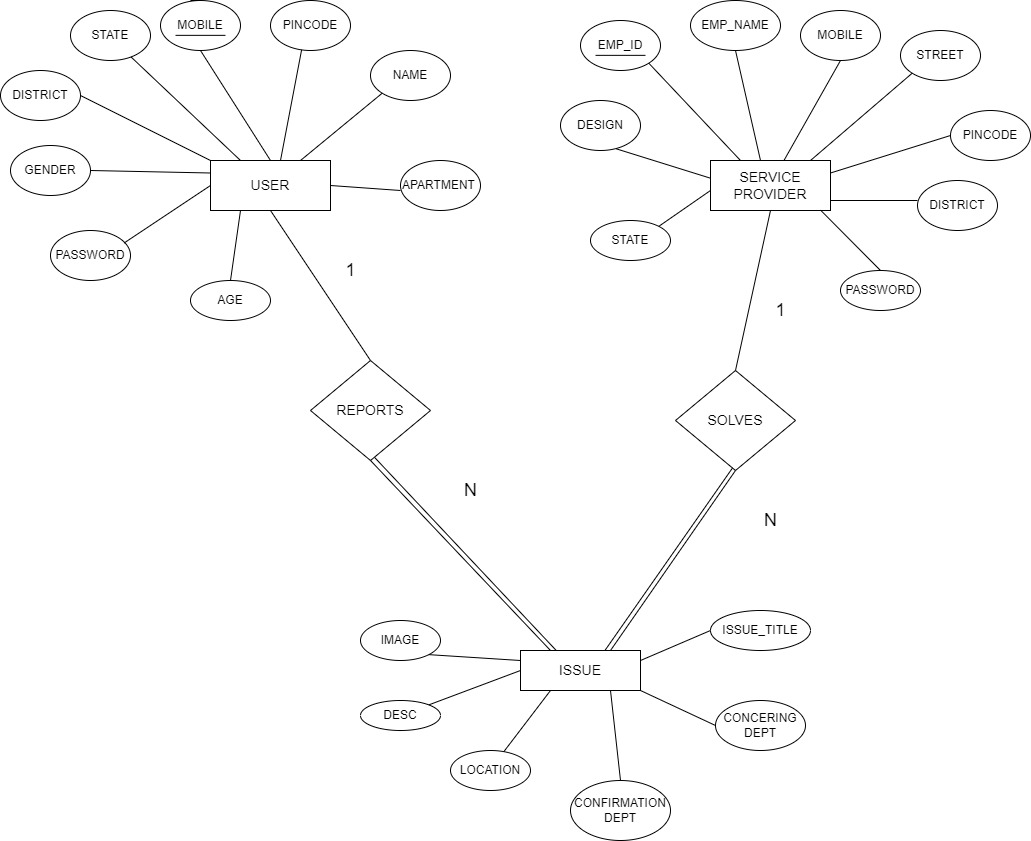
\includegraphics[width=6in,height=3.5in]{ER.jpg}
\caption{ER Diagram for Grievance Portal Management System}
\end{figure}
\newpage
\section{Mapping From ER Diagram to Schema Diagram}
Figure 3.2 represent the relational schema of the proposed system.
\begin{itemize}
\item\textbf{Mapping of regular entity types:}
For each entity we have created the table i.e user,service provider and issue.
\item\textbf{Mapping of weak entity types:}
A weak entity set is one which does not have any primary key associated with it.In this relational schema there is no weak entity type.
\item\textbf{Mapping of Binary 1:1 Relation Types:}
In relational database design,there is no 1:1 Relationship.
\item\textbf{Mapping of Binary 1:N Relationship Types:}
In case both entities in a 1:1 binary relationship are in total participation, then merge both entity types into one (usually in the name of the relationship). For each binary 1:N relationships, identify the relation S that represents the entity type on the N side.in this relational schema there is  1:n relation between space-station and crew, space station and component.
\item\textbf{Mapping of Binary M:N Relationship Types:}
In relational database design,there is no M:N Relationship.
\item\textbf{Mapping of Multi-valued attributes:}
For each multi-valued attribute A, create a new relation R.This relation R will include an attribute corresponding to A, plus the primary key attribute K-as a foreign key in R-of the relation that represents the entity type of relationship type that has A as an attribute.Here there is no multi-valued attribute.
\item\textbf{Mapping of N-ary Relationship Types:}
For each n-ary relationship type R, where n is greater than 2, create a new relationship S to represent R.
Include as foreign key attributes in S the primary keys of the relations that represent the participating entity types. 
Also include any simple attributes of the n-ary relationship type (or simple components of composite attributes) as attributes of S.Here there is no such N-ary relationship type
\end{itemize}
\newpage
\section{Assumptions}
\begin{itemize}
	\item One service provider can solve any number of issues.
	\item User can drops their complaint in issue table.
	\item Service provider gets to know at which particular location the issue has been reported.
	
\end{itemize}
\section{Schema Diagram}
A Schema is a pictorial representation of the relationship between the database tables in the database that is created. The database schema of a database system is its structure described in a formal language sup ported by the database management system (DBMS). A database schema defines its entities and the relationship among them.A database schema contains schema objects that may include tables, fields, relationships, primary key, foreign key. It provides knowledge about how the data is organized in a database and how it is associated with other data.The schema does not physically contain the data itself; instead, it gives information about the shape of data and how it can be related to other tables or models.
\begin{figure}[hbtp]
\centering
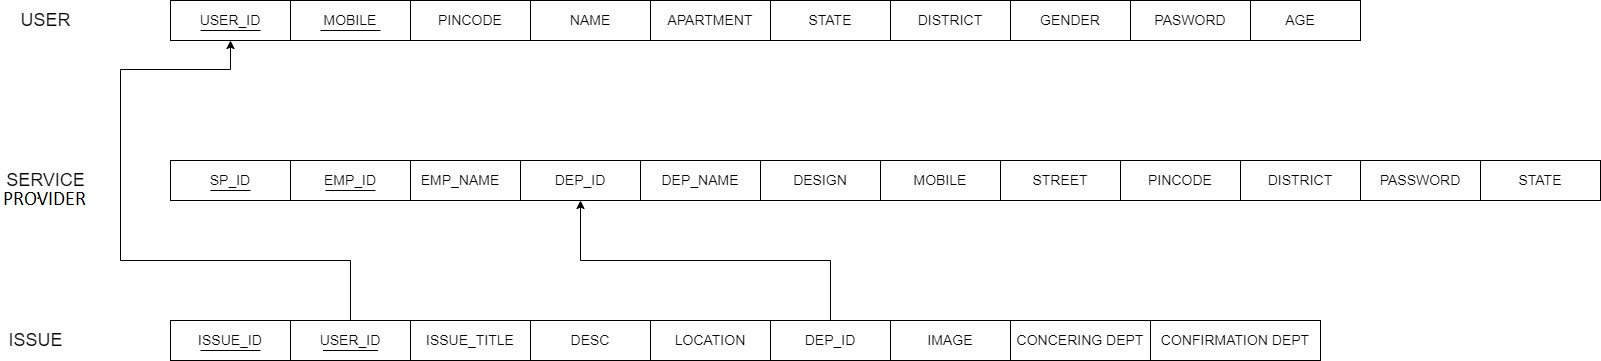
\includegraphics[width=6.5in,height=2in]{godzi.jpg}
\caption{Schema Diagram for Grievance Portal Management System}
\end{figure}
\chapter{Implementation}
\section{Pseudo-Codes Used}
\noindent\textbf{Pseudocode used for view:}\\
The below php code is for view of the data into the database. Here the admin can view the users entire details.\\
\begin{figure}[hbtp]
\centering
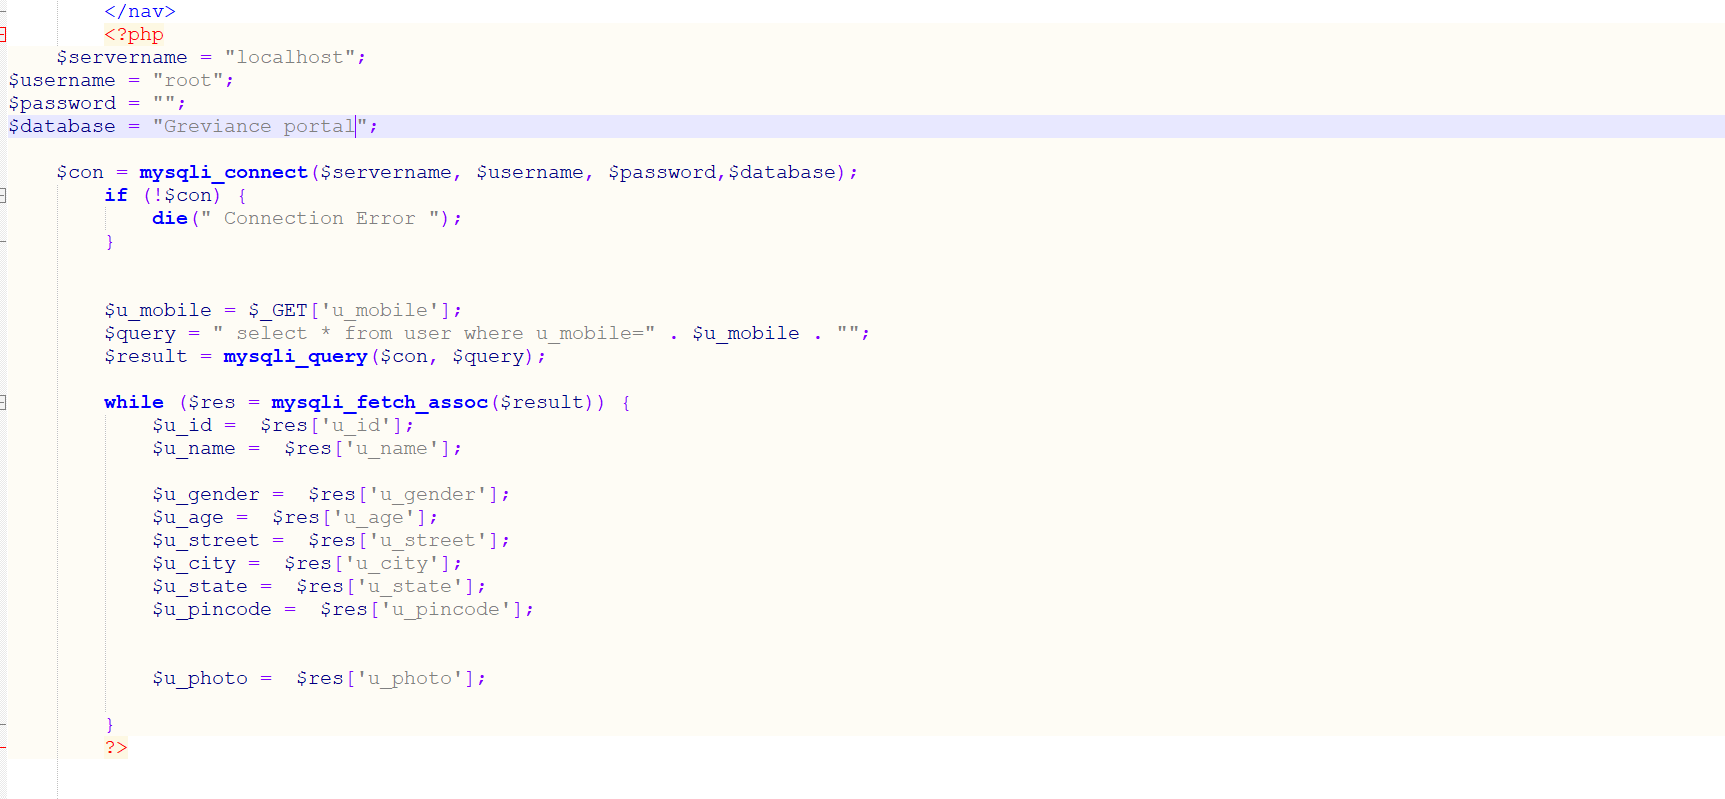
\includegraphics[width=6.4in,height=2in]{view.png}
\caption{Pseudocode for View }
\end{figure}
\newpage
\noindent\textbf{Pseudocode used for deletion:}\\
The below php code is for deletion of the data from the database. If the admin clicks on the delete button the entire tuple gets deleted and gives a pop up message.
\begin{figure}[hbtp]
\centering
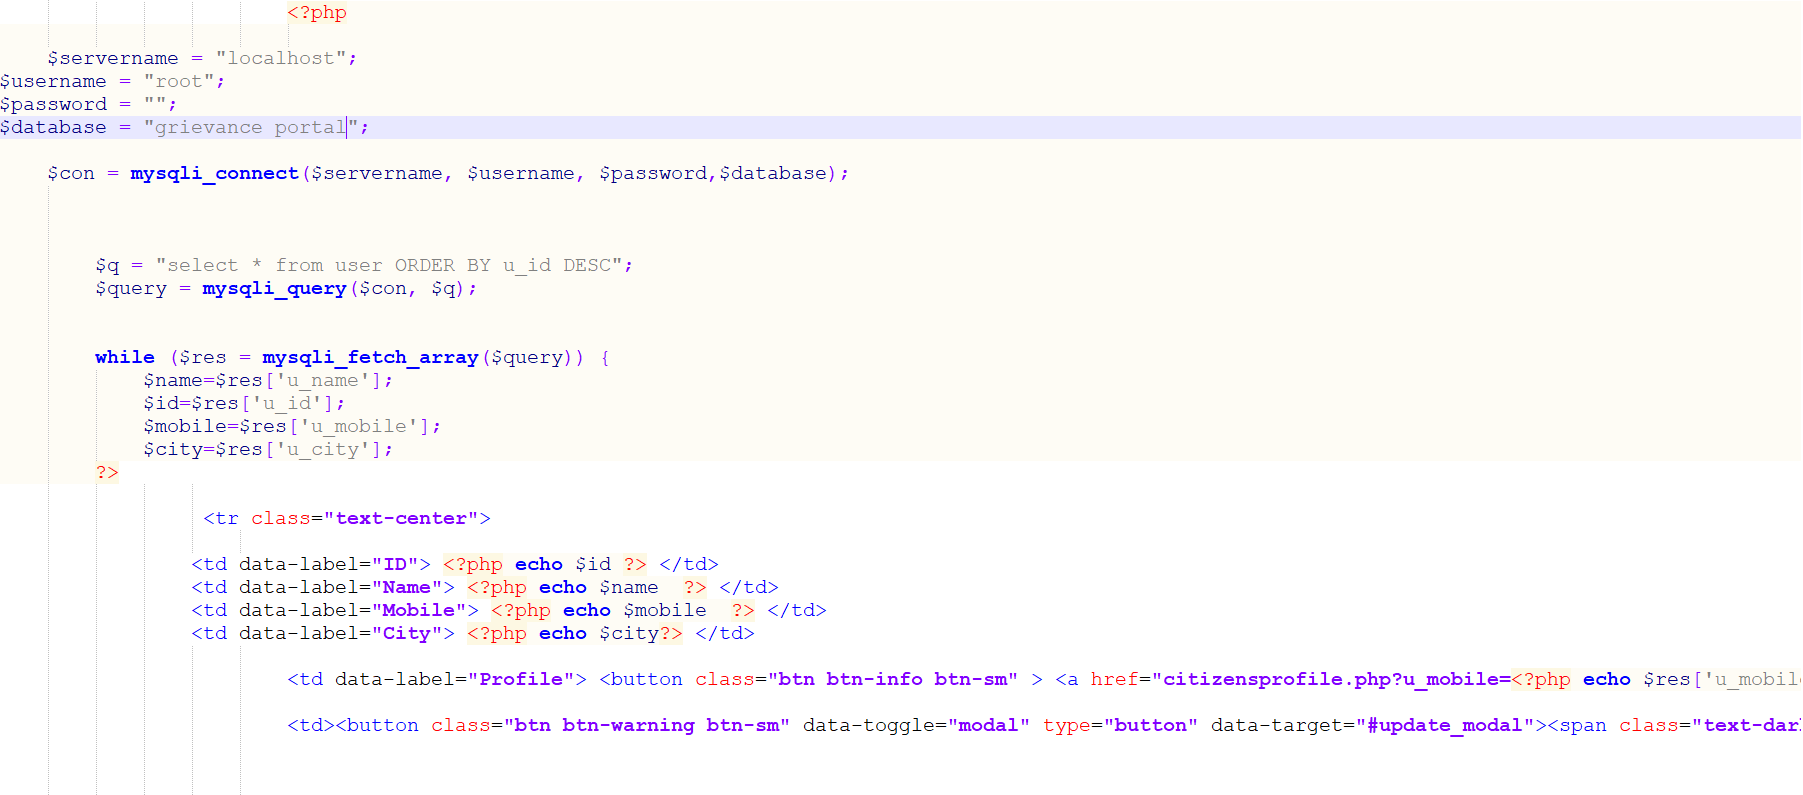
\includegraphics[width=6.4in,height=3in]{update.png}
\caption{Pseudocode code for deletion }
\end{figure}

\noindent \textbf {Pseudocode used for updation:}
The below php code is for updation of the data in the database.Here the admin can update the details of the user.
\begin{figure}[hbtp]
\centering
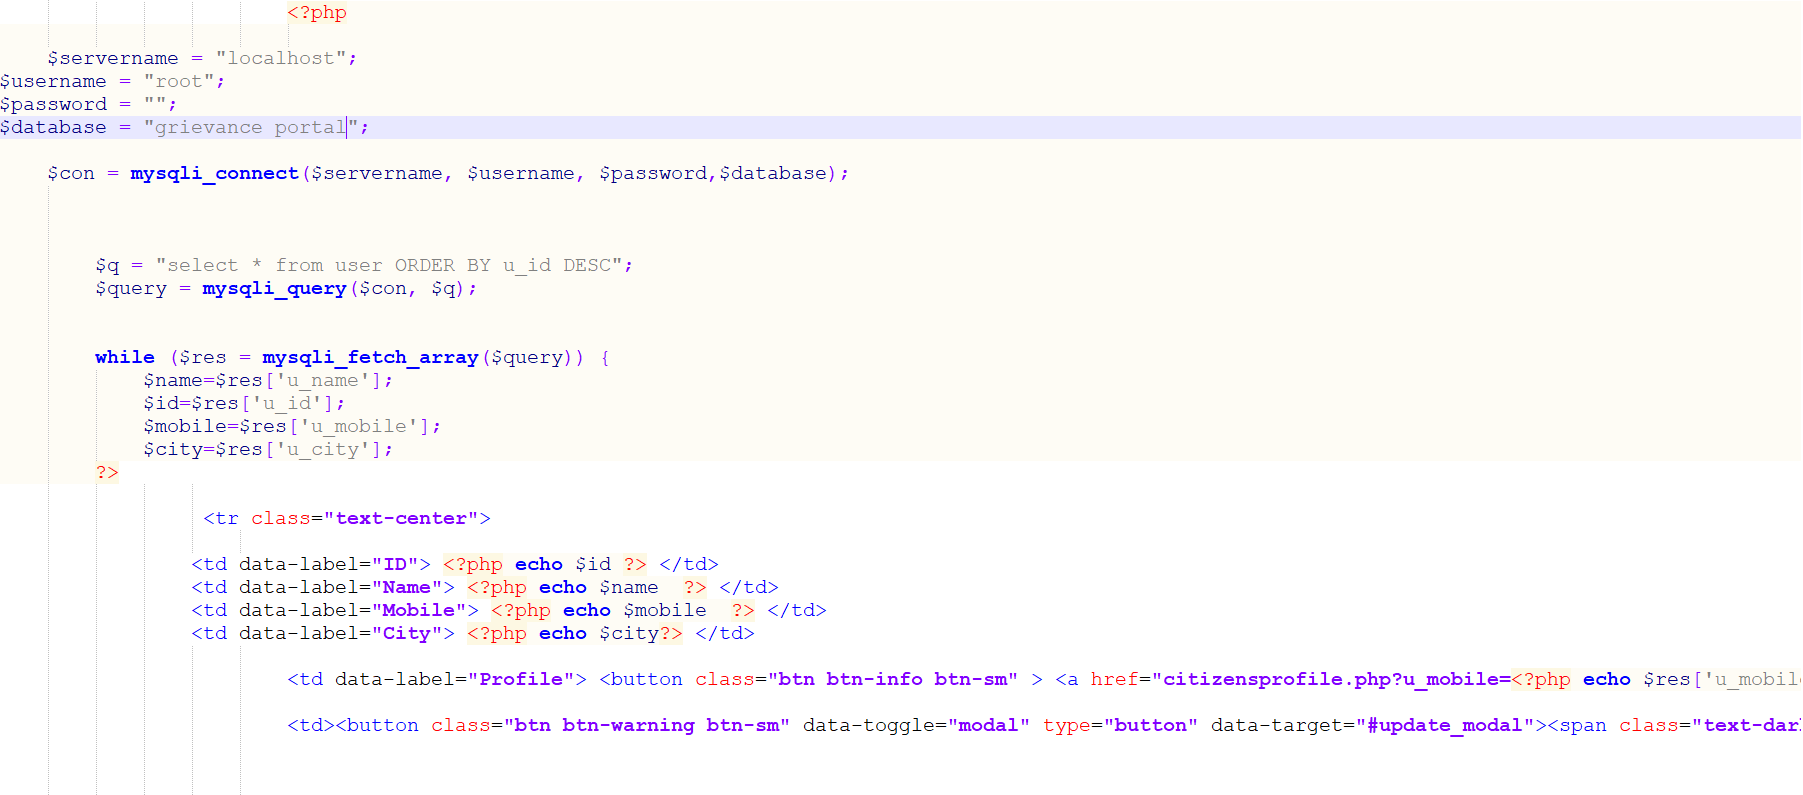
\includegraphics[width=6.4in,height=3in]{update.png}
\caption{Pseudocode for updation }
\end{figure}
\newpage
\section{Tables Used}
\textbf{Admin Table:}
Here we create a table named admin having attributes aid, aname,password and aid as the primary key.
\begin{figure}[hbtp]
\centering
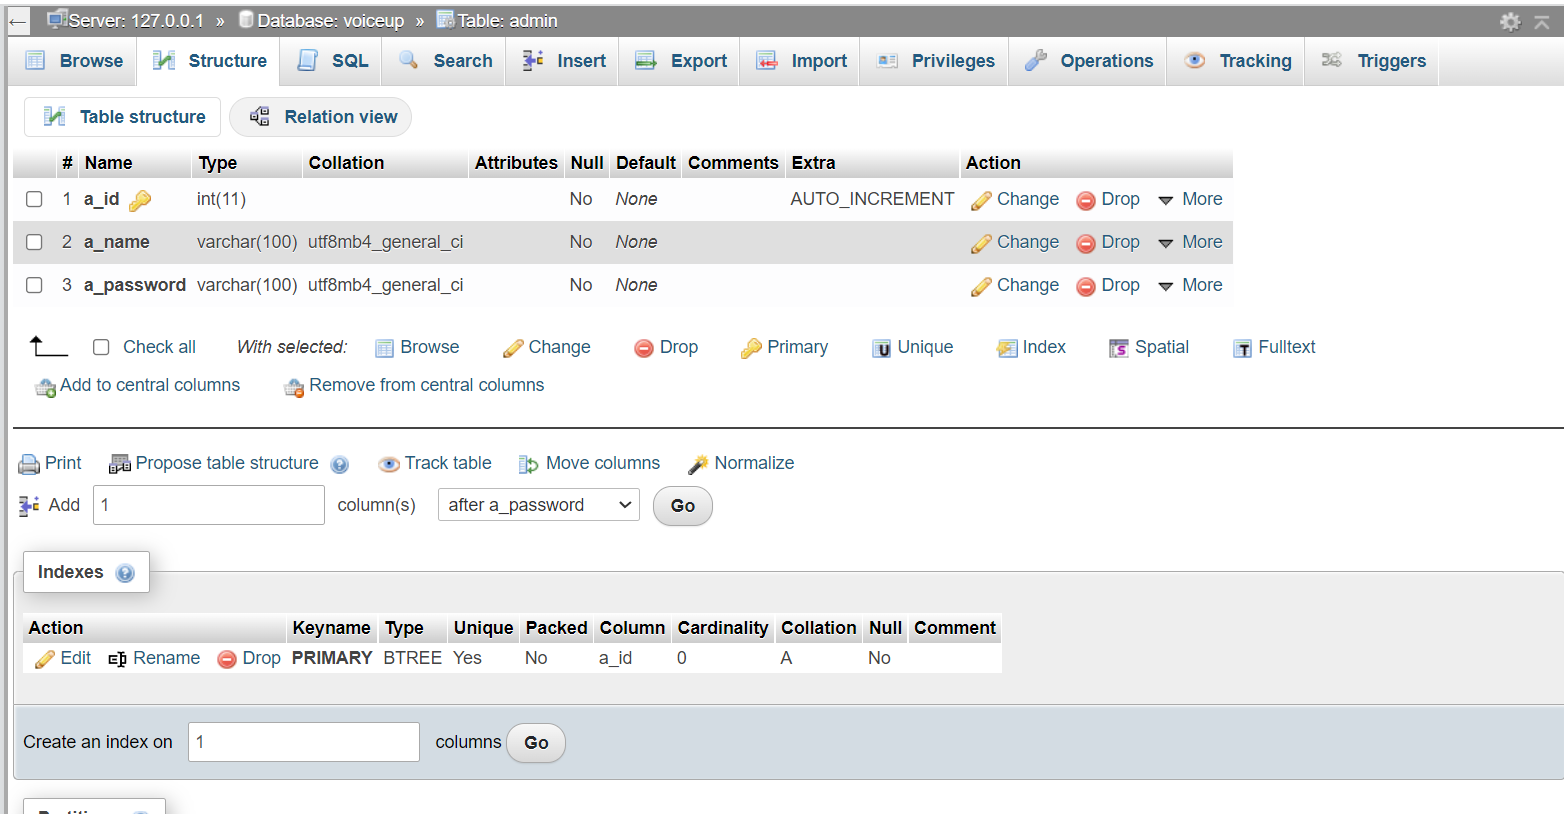
\includegraphics[width=6.4in,height=2.7in]{fa.png}
\caption{Structure of Admin table}
\end{figure}

\noindent\textbf{Contact us Table:}
Here we create a table named contactus having attributes cid, cname, cmobile, cemail ,caddress ,cmessage. Here cid is the primary key.\\
\begin{figure}[hbtp]
\centering
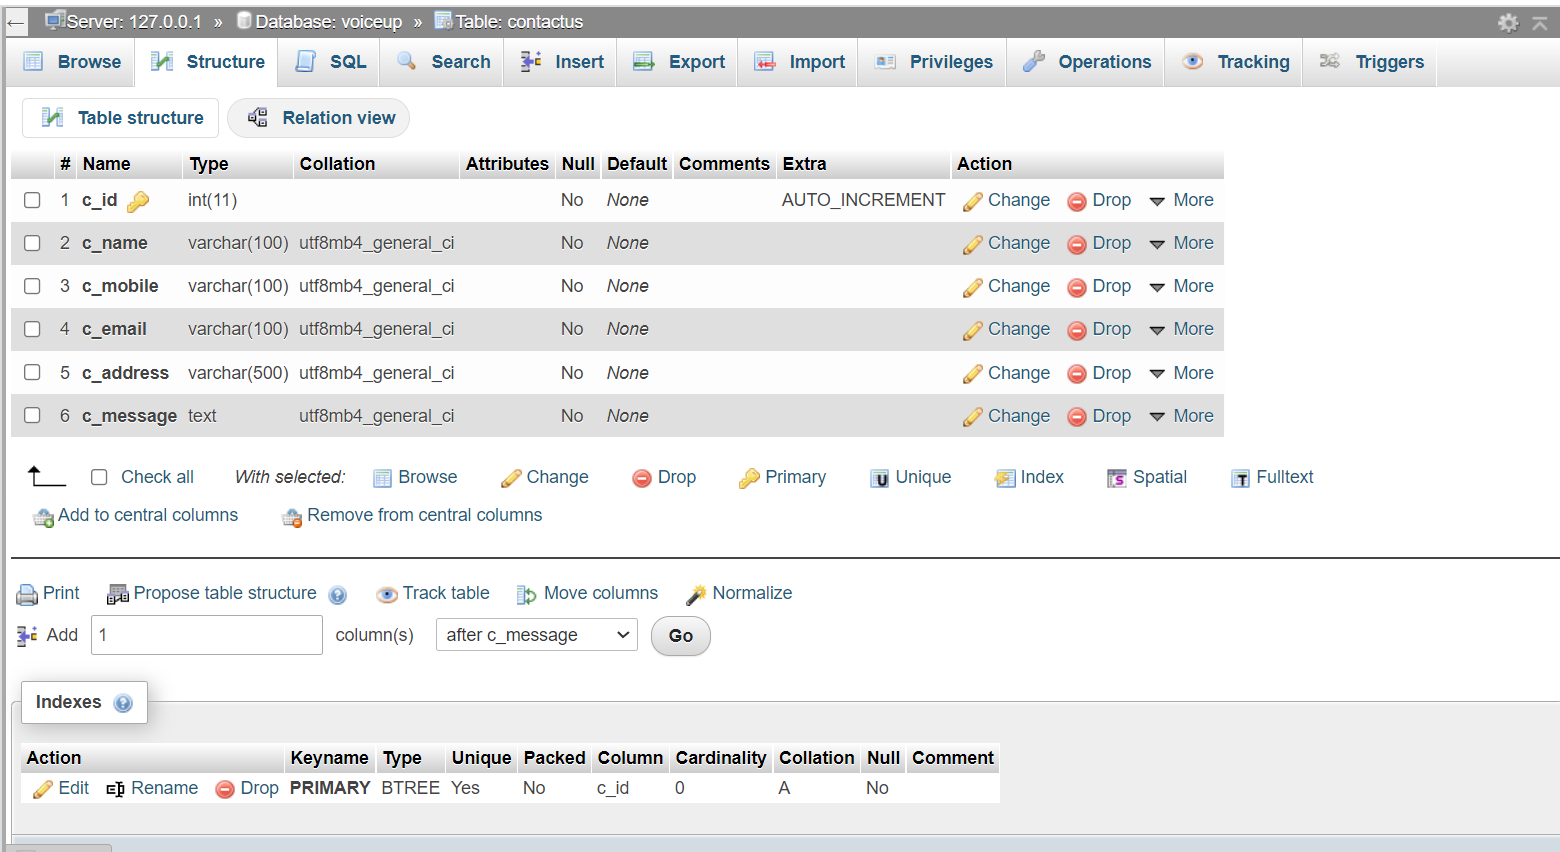
\includegraphics[width=6.4in,height=2.7in]{fc.png}
\caption{Structure of  Contact us table}
\end{figure}
\vspace{2.5in}

\noindent\textbf{Service provider Table:}
Here we create a table named dept having attributes $d\_id$ , $d\_type$ ,$d\_mobile$,$d\_street$,$d\_city$,$d\_state$,$d\_pincode$,$d\_cpname$ ,$d\_cppos$,$d\_cpeid$,password. Here $d\_id$  is the primary key and  $d\_mobile$ is the foreign key that references $u\_mobile$ of the user table.\\

\begin{figure}[hbtp]
\centering
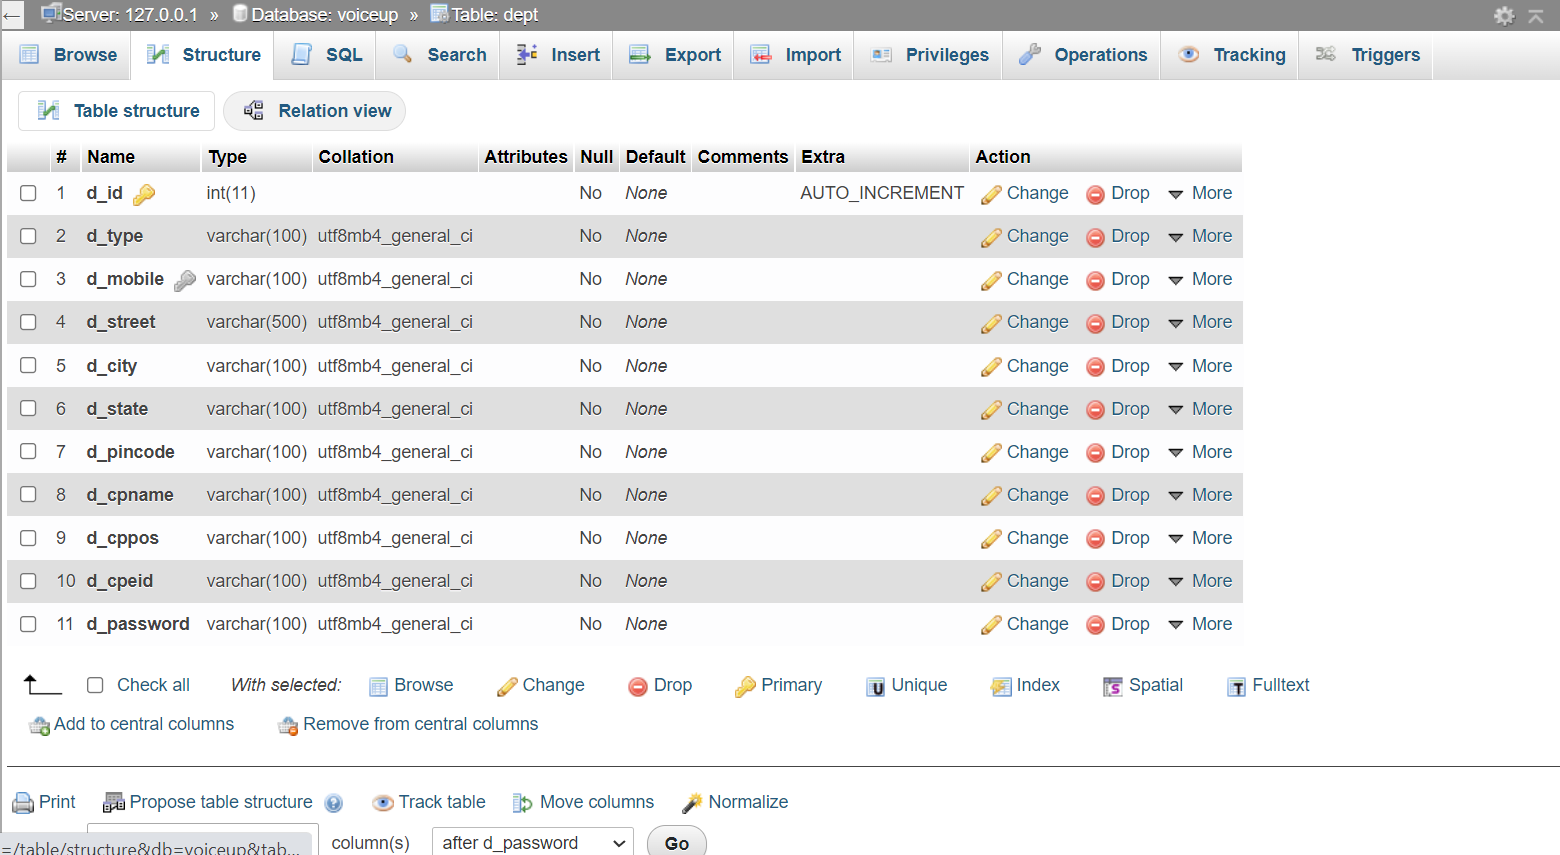
\includegraphics[width=6.4in,height=2.7in]{fd.png}
\caption{Structure of Serviceprovider table}
\end{figure}
\noindent \textbf{Issue Table:}
Here we create a table named issue having attributes $i\_id$ , $i\_uid$ ,$i\_type$ , $i\_title$ ,$i\_des$ ,$i\_exactloc$,$i\_date$ , $i\_date$ , $i\_img1$ , $i\_status$ , $i\_idid$. Here $i\_id$ is the primary key and $u\_id$ is the foreign key that references $user\_id$ of the user table.\\

\begin{figure}[hbtp]
\centering
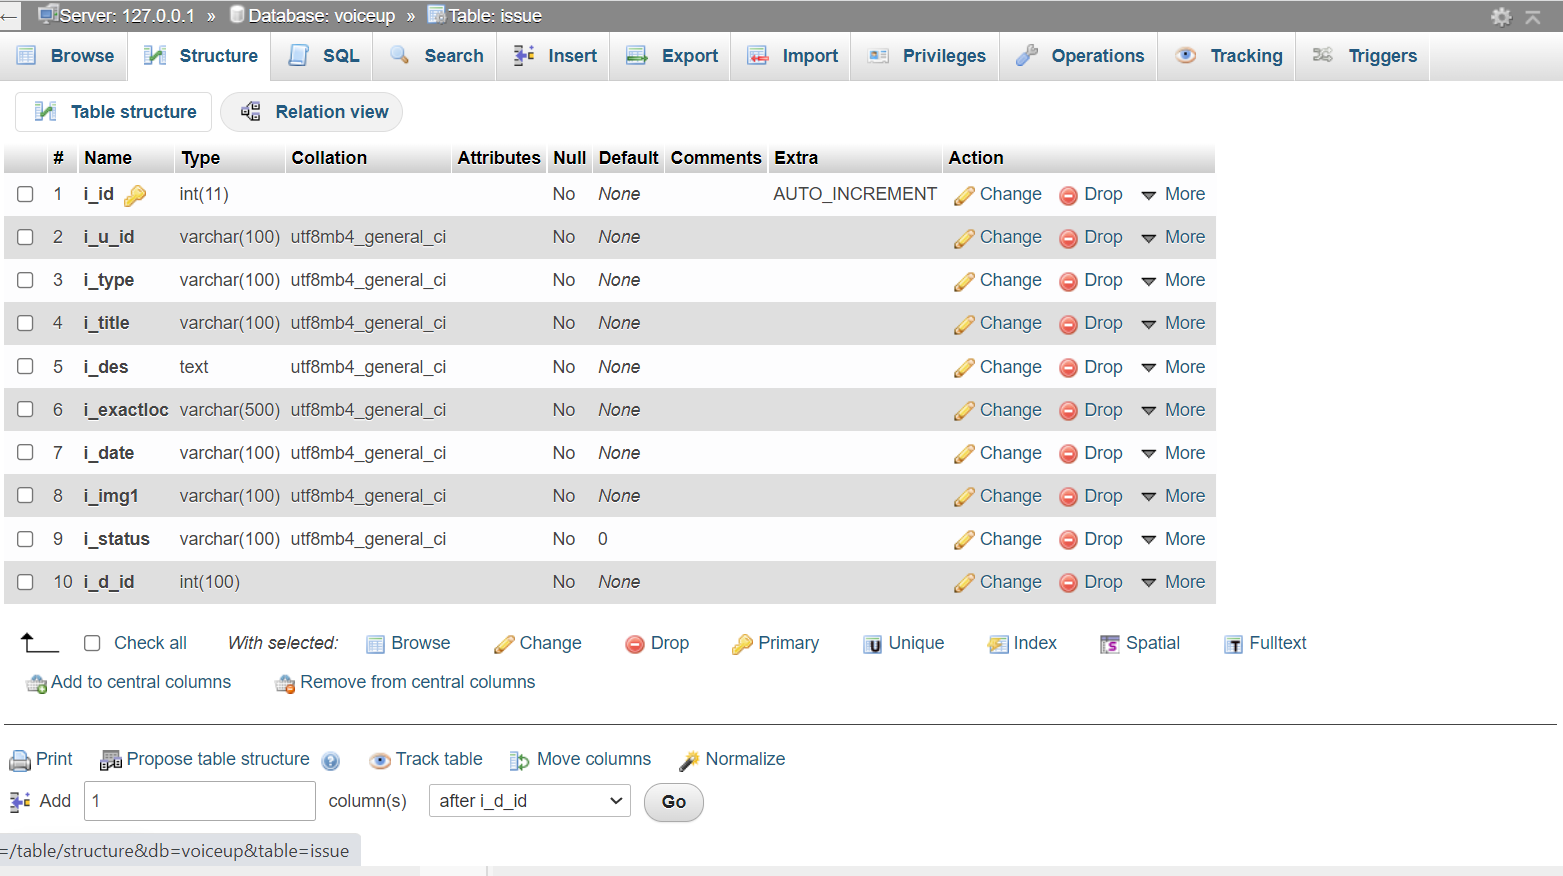
\includegraphics[width=6.4in,height=2.7in]{fi.png}
\caption{Structure of Issue table}
\end{figure}
\vspace{2in}
\noindent \textbf{User Table:}
Here we create a table named user having attributes $u\_id$ , $u\_mobile$ , $u\_name$, $u\_gender$ , $u\_age$ , $u\_street$ , $u\_city$ , $u\_state$ , $u\_pincode$ , $u\_password$. Here $u\_id$ and $u\_mobile$  are the primary keys.
\begin{figure}[hbtp]
\centering
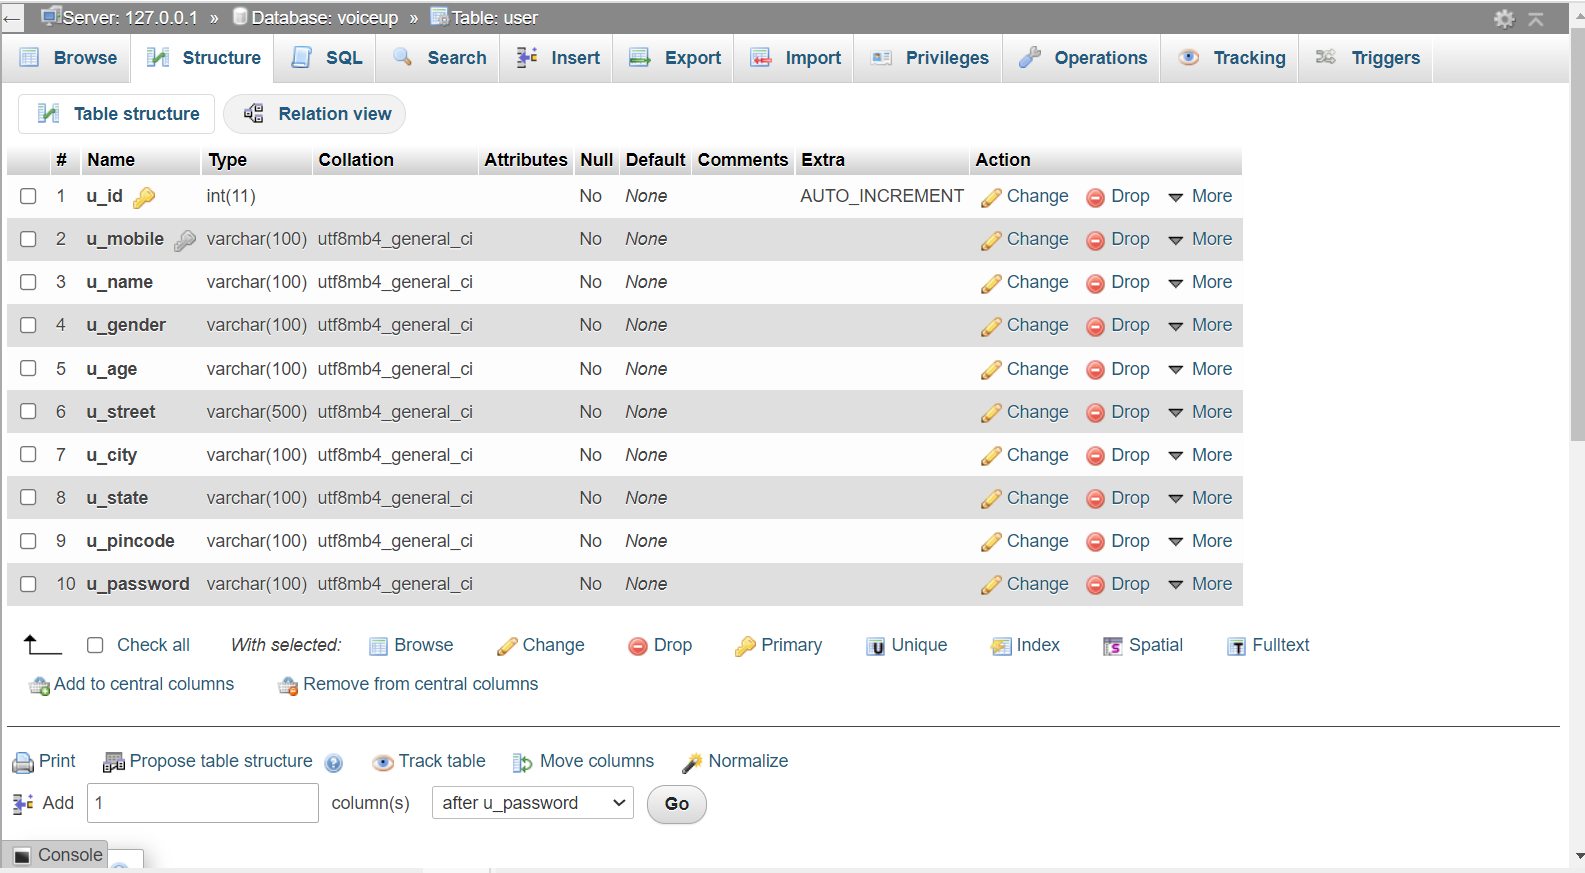
\includegraphics[width=6.4in,height=3in]{fu.png}
\caption{Structure of User table}
\end{figure}
\vspace{2.50in}

\chapter{Results and Disscussion}
% \section{Admin operations:}
% This page allows the admin to select and perform a particular operation in the database. The admin will select any one of the module from the given five modules and perform various operations.
% \vspace{0.10in}
% \begin{figure}[hbtp]
% \centering
% 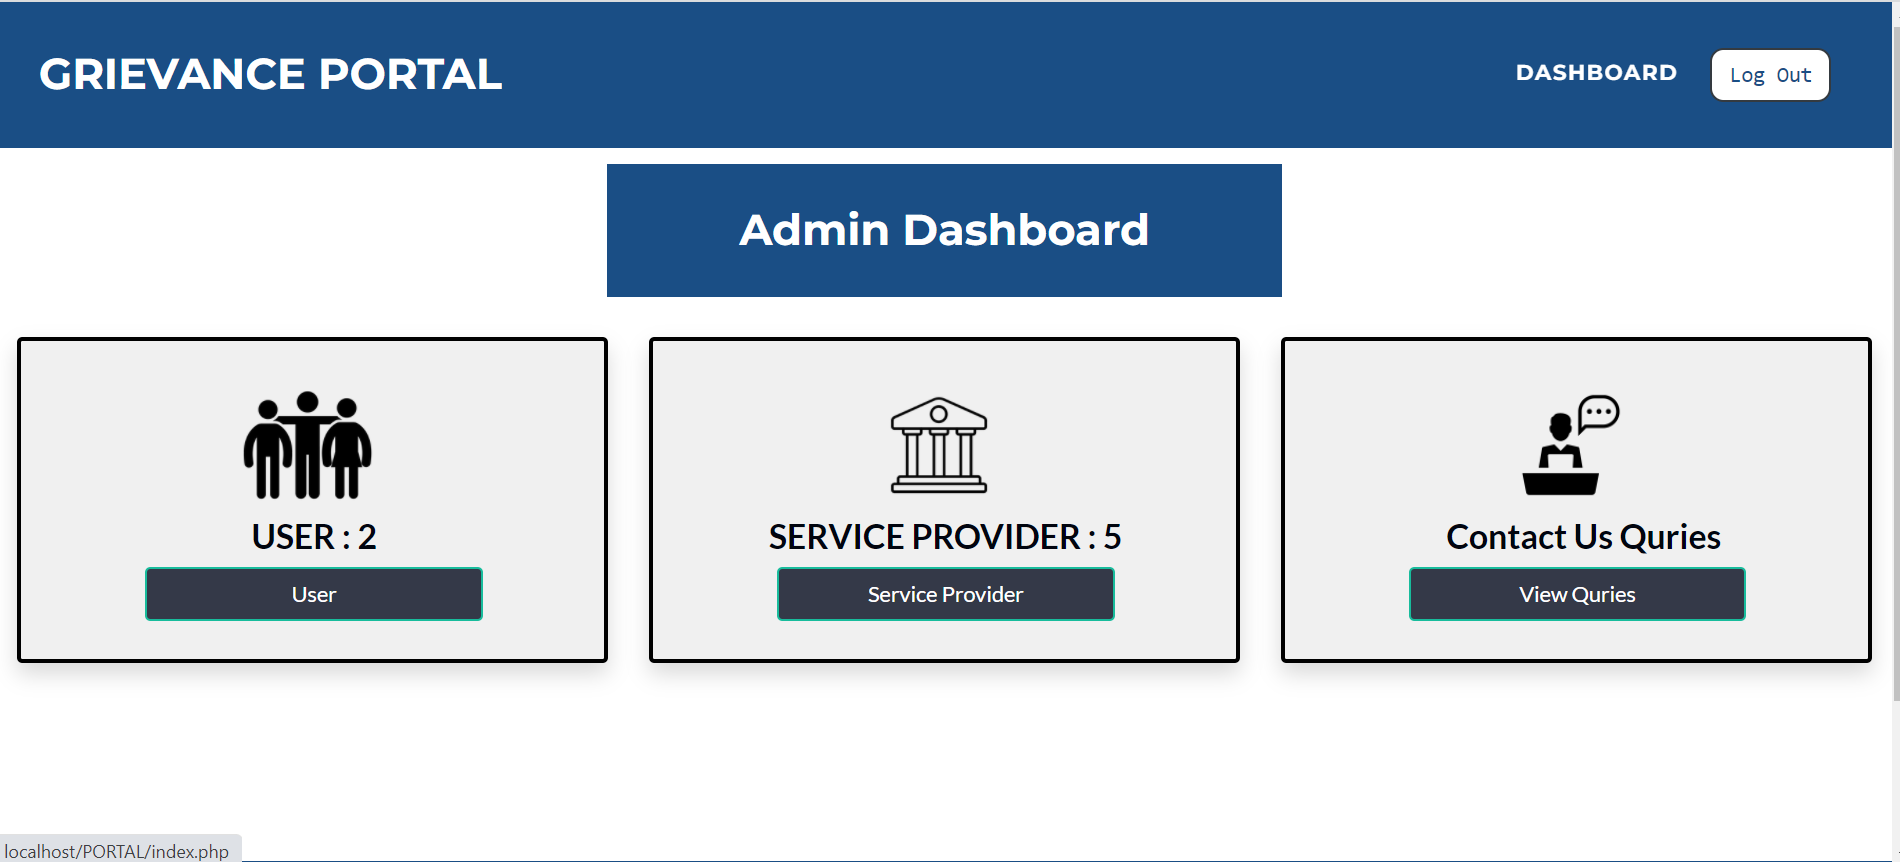
\includegraphics[width=6in,height=3in]{admin1.png}
% \caption{Admin operations}
% \end{figure}
\section{User Details}
This page allows the admin to add the details of the space station to the database.
\begin{figure}[hbtp]
\centering
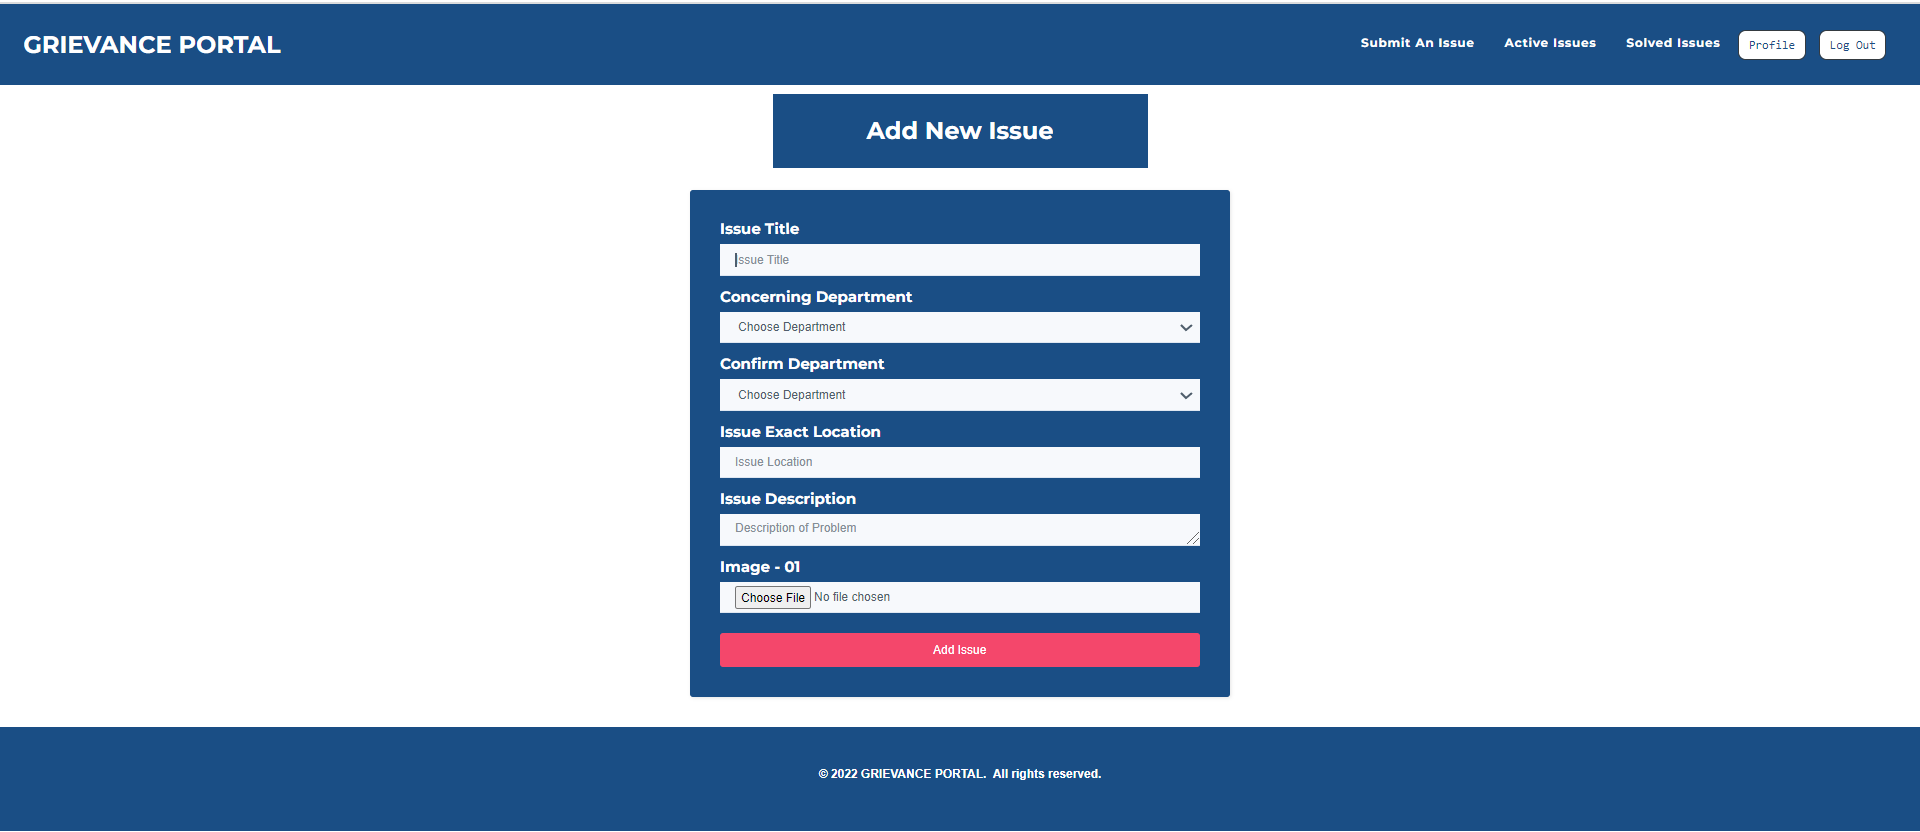
\includegraphics[width=6in,height=3in]{user.png}
\caption{User Details}
\end{figure}
\vspace{0.10in}
\newpage
\section{Service Provider Details}
This page allows the admin to add the details of the base station to the database.
\begin{figure}[hbtp]
\centering
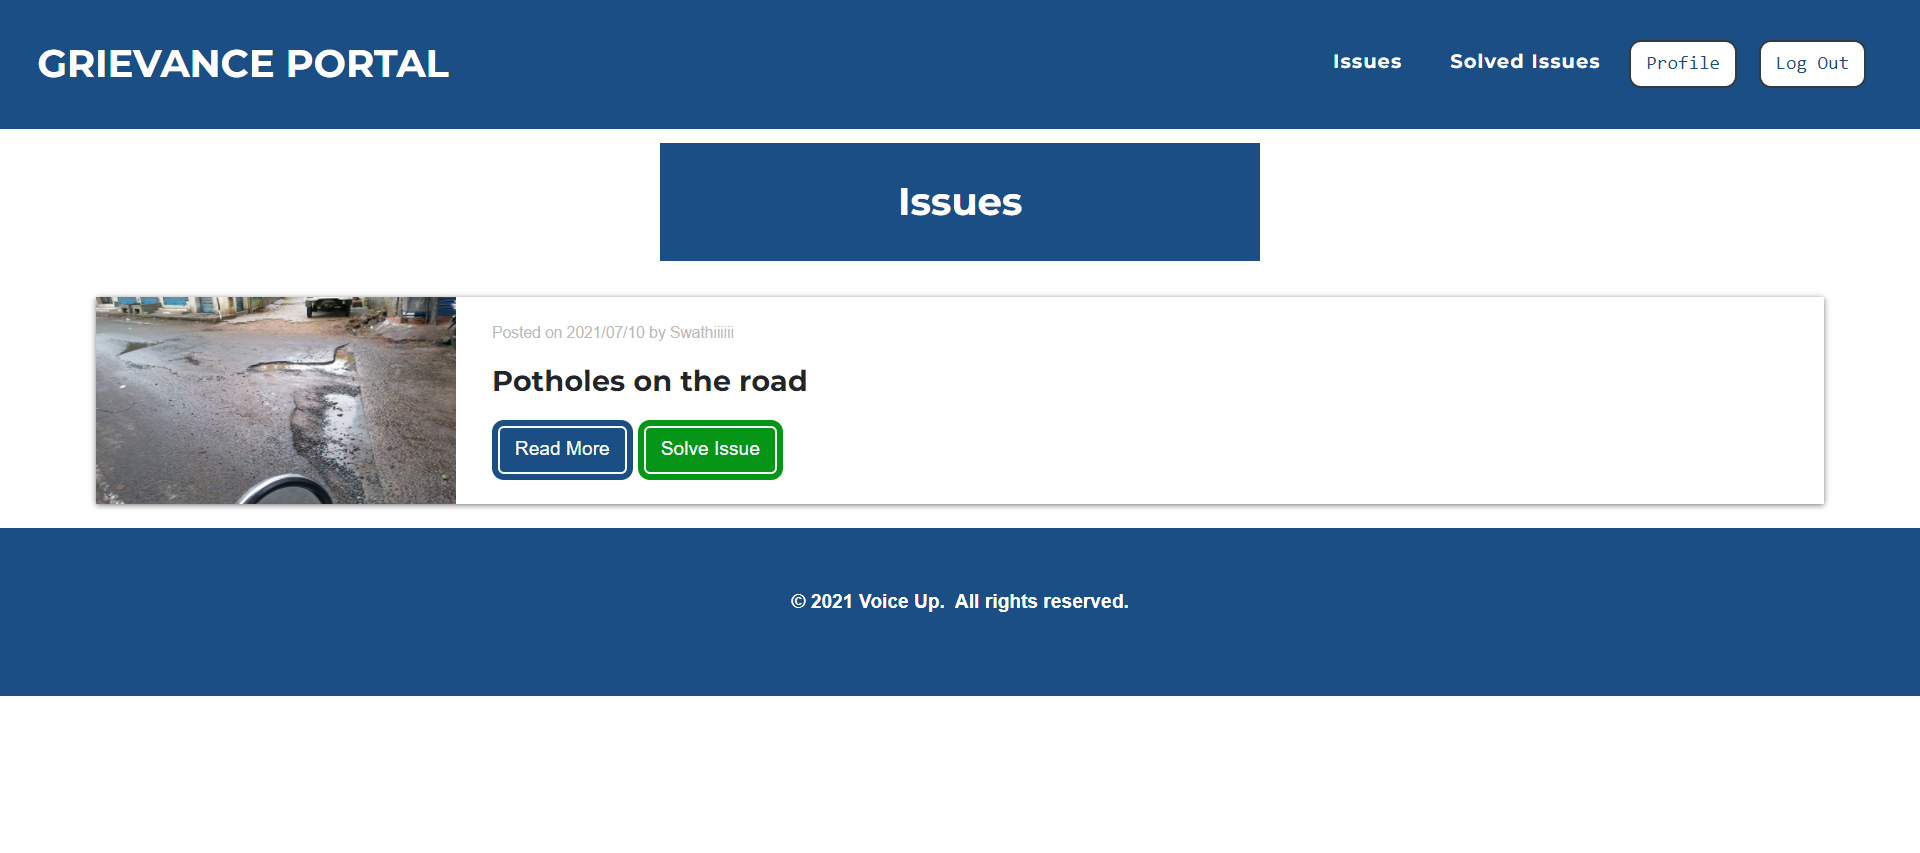
\includegraphics[width=6in,height=3in]{sp.png}
\caption{Service Provider Details}
\end{figure}
\section{Solved Issue Details}
This page allows the admin to add, delete and update crew details to the database.
\begin{figure}[hbtp]
\centering
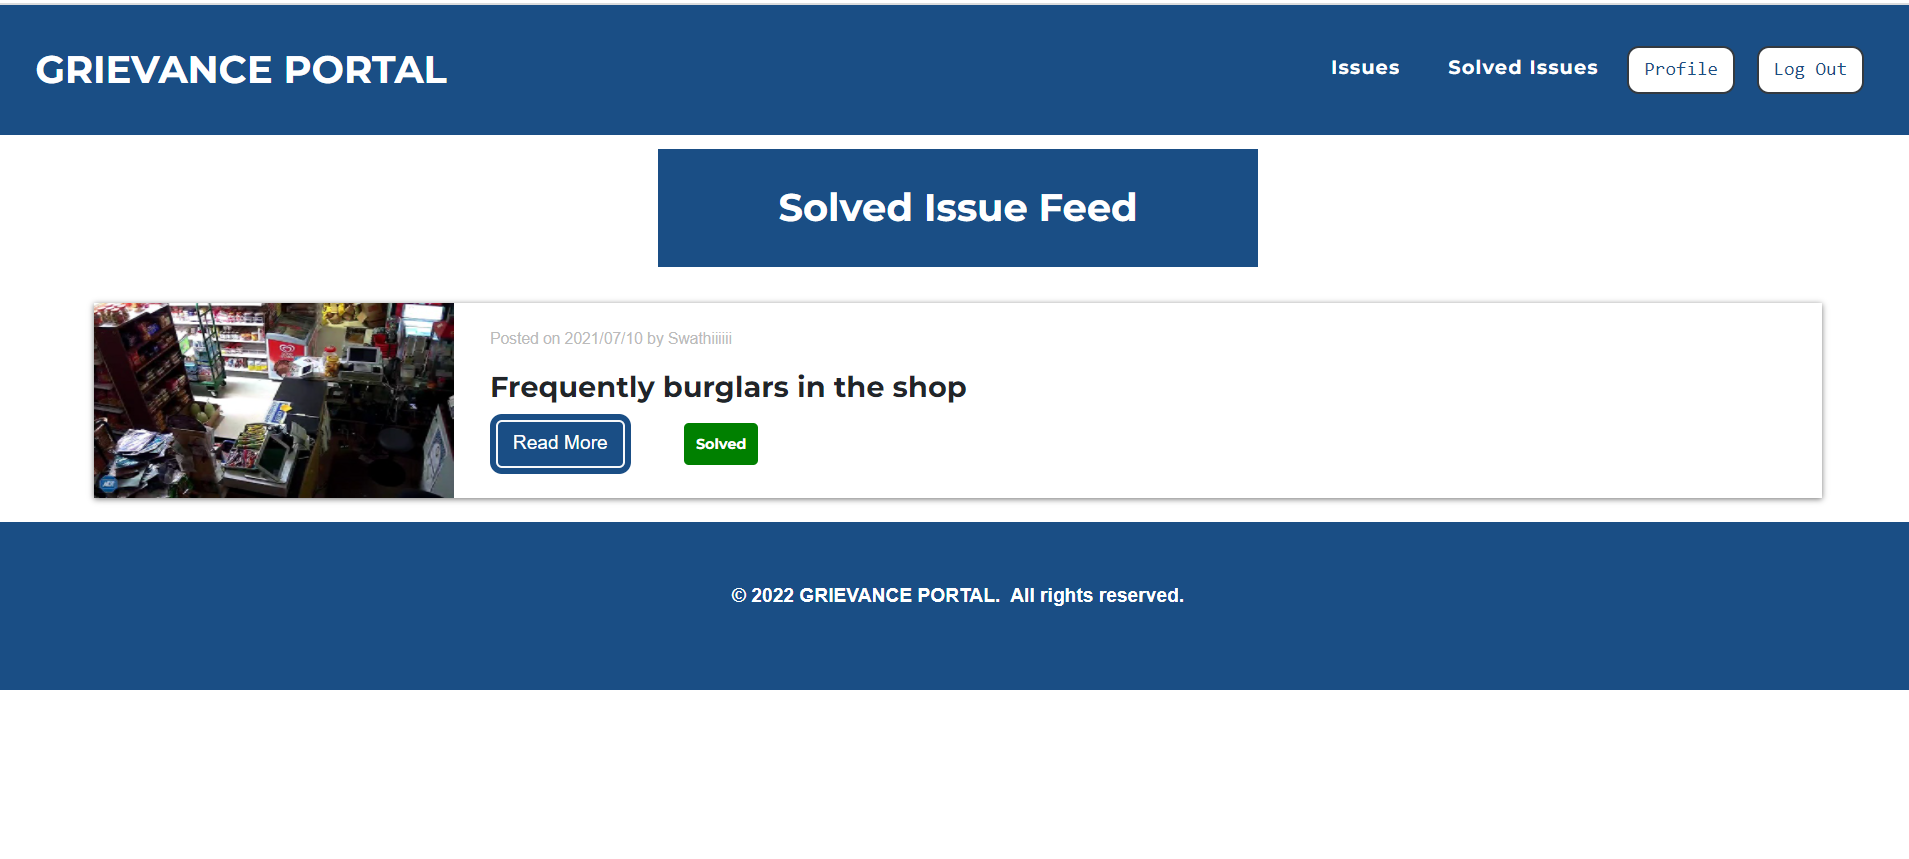
\includegraphics[width=6in,height=3in]{sissue.png}
\caption{Solved Issue  Details}
\end{figure}
\section{Unsolved Issue Details}
Looking at the components available this page allows the admin to add, delete and update component details to the database
\begin{figure}[hbtp]
\centering
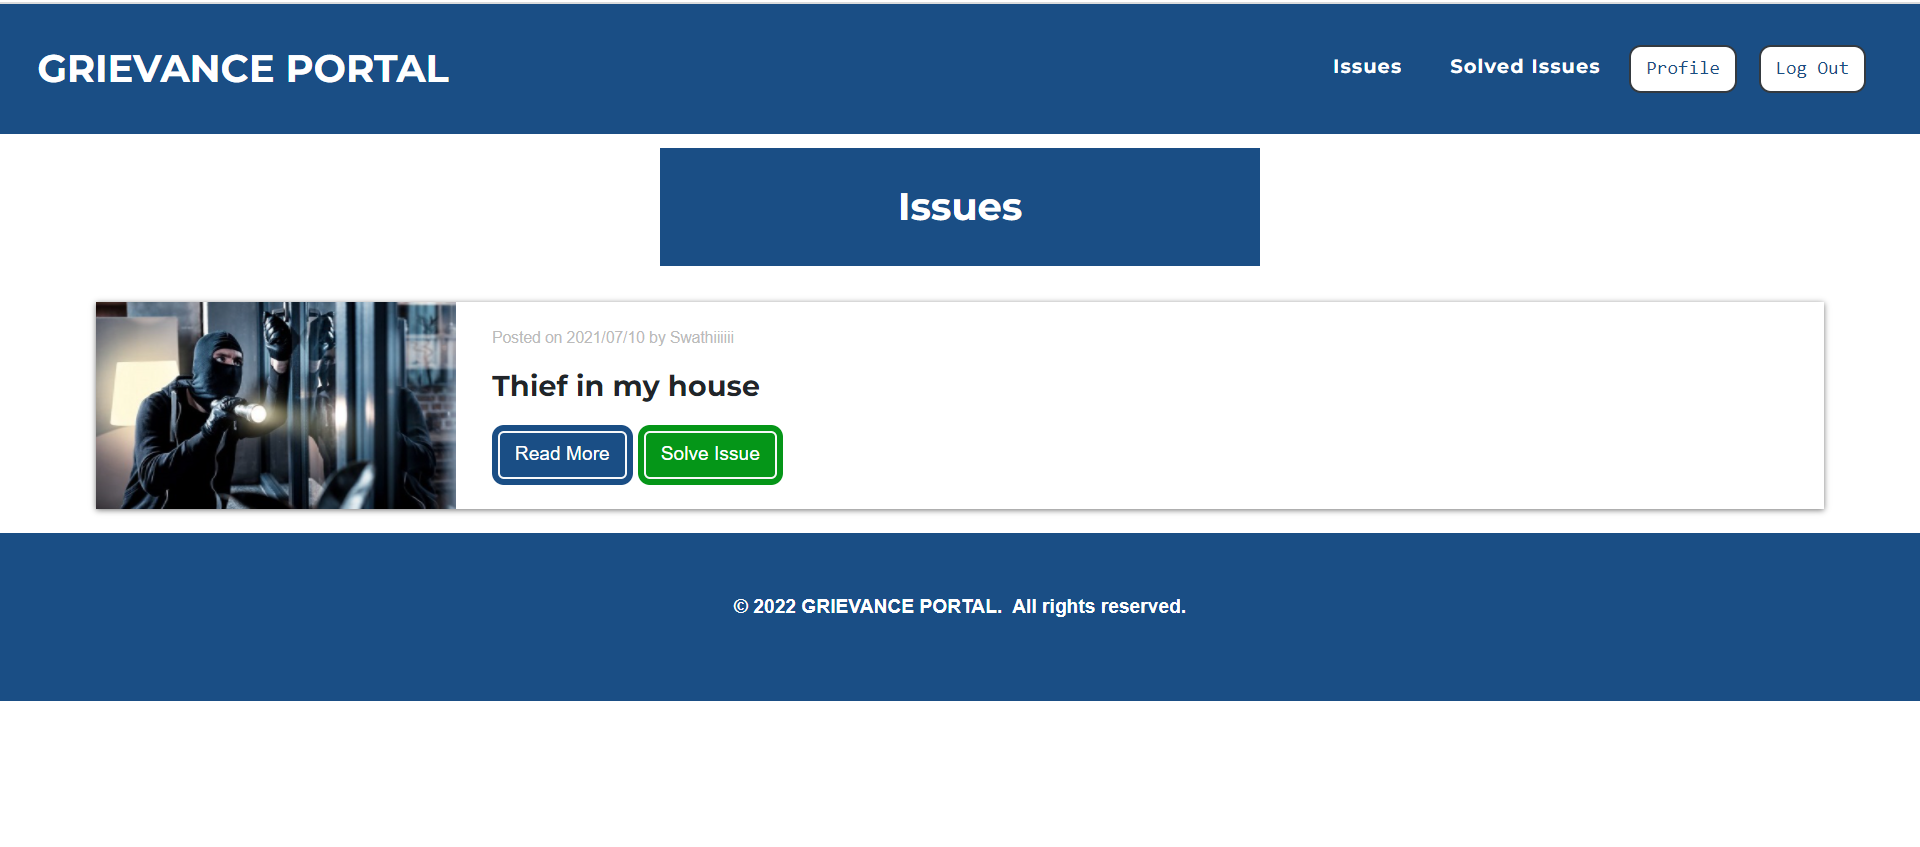
\includegraphics[width=6in,height=3in]{cissue.png}
\caption{Unsolved Issue Details}
\end{figure}.
\vspace{1in}
% \section{Contact Us Details}
% This page allows the admin to maintain the records of the components that is supplied and needs to be supplied to the space station from base station.
% \vspace{0.2in}
% \begin{figure}[hbtp]
% \centering
% 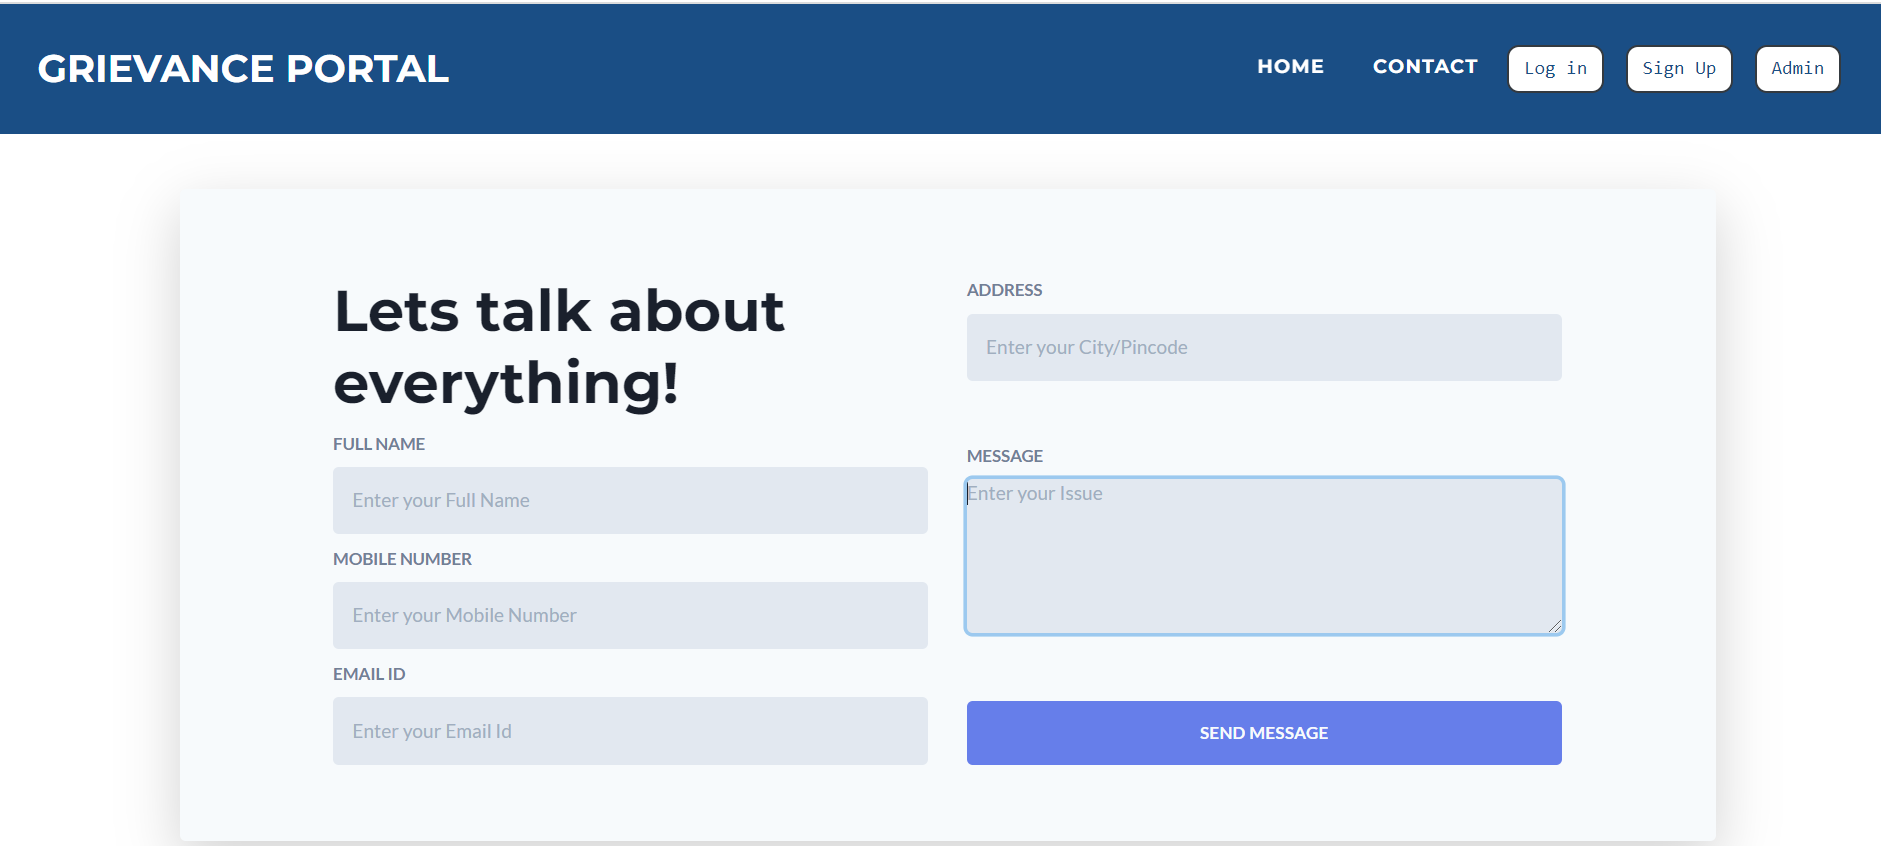
\includegraphics[width=6in,height=3in]{cus.png}
% \caption{Contact Us  Details}
% \end{figure}
\chapter{Conclusion and Future work}
This project is available to all users to submit their grievances and it helps them in obtaining the desired solution by tracking the exact location at which particular location the grievance is being registered.This project acts a bridge between the user and service providers. This portal can be accessed by the user without any issues. This portal is user friendly and user can access this portal anytime.
\newpage
\pagestyle{plain}
\renewcommand{\bibname}{References}
\bibliography{references}
\addcontentsline{toc}{chapter}{References}
\begin{thebibliography}{35}
\bibitem{ds}Database systems Models, Languages, Design and Application Programming, Ramez Elmasri and Shamkant B. Navathe, 7th Edition, Pearson.

\bibitem{dm}Database management systems, Ramakrishnan, and Gehrke, 3rd Edition, 2014, McGraw Hill.

\bibitem{korth}Silberschatz Korth and Sudharshan: Database System Concepts, 6th Edition, Mc-Graw Hill, 2013.

\bibitem{mor}Coronel, Morris, and Rob, Database Principles Fundamentals of Design, Implementation and  
Management, Cengage Learning 2012.

\end{thebibliography}

\end{document}